\documentclass[11pt,a4paper]{article}

% ── Packages ──────────────────────────────────────────────────────────────────
\usepackage[margin=2.5cm]{geometry}
\usepackage[utf8]{inputenc}
\usepackage[T1]{fontenc}
\usepackage{lmodern}
\usepackage{microtype}
\usepackage{booktabs}
\usepackage{graphicx}
\usepackage{xcolor}
\usepackage{hyperref}
\usepackage{amsmath}
\usepackage{multirow}
\usepackage{array}
\usepackage{makecell}
\usepackage{caption}
\usepackage{subcaption}
\usepackage{enumitem}
\usepackage{titlesec}
\usepackage{abstract}
\usepackage{fancyhdr}
\usepackage{footnote}

% ── Colors ────────────────────────────────────────────────────────────────────
\definecolor{l1red}{RGB}{220,53,69}
\definecolor{l2yellow}{RGB}{255,193,7}
\definecolor{l3green}{RGB}{40,167,69}
\definecolor{deltacolor}{RGB}{214,39,40}
\definecolor{lightgray}{RGB}{248,249,250}

% ── Hyperref ──────────────────────────────────────────────────────────────────
\hypersetup{
  colorlinks=true,
  linkcolor=blue!60!black,
  citecolor=blue!60!black,
  urlcolor=blue!60!black,
}

% ── Section formatting ────────────────────────────────────────────────────────
\titleformat{\section}{\large\bfseries}{\thesection.}{0.5em}{}
\titleformat{\subsection}{\normalsize\bfseries}{\thesubsection}{0.5em}{}

% ── Caption formatting ────────────────────────────────────────────────────────
\captionsetup{font=small, labelfont=bf, width=0.92\textwidth}

% ── Header ────────────────────────────────────────────────────────────────────
\pagestyle{fancy}
\fancyhf{}
\rhead{\small S-OWMI V1 — Apart Research Global South AI Safety Hackathon, June 2026}
\rfoot{\small\thepage}
\renewcommand{\headrulewidth}{0.4pt}

% ── Column type for fixed-width centered ──────────────────────────────────────
\newcolumntype{C}[1]{>{\centering\arraybackslash}p{#1}}

% ── Helpers ───────────────────────────────────────────────────────────────────
\newcommand{\lvlone}{\textcolor{l1red}{\textbf{L1}}}
\newcommand{\lvltwo}{\textcolor{l2yellow}{\textbf{L2}}}
\newcommand{\lvlthree}{\textcolor{l3green}{\textbf{L3}}}
\newcommand{\sig}[1]{\textbf{#1}}   % bold for significant p-values
\newcommand{\dasr}{$\Delta$ASR}

% ──────────────────────────────────────────────────────────────────────────────
\begin{document}

% ── Title block ───────────────────────────────────────────────────────────────
\begin{center}
  {\LARGE\bfseries S-OWMI: A Perimeter Auditing Framework for\\[4pt]
    Open-Weight Models in Latin American Institutions}\\[1.2em]
  {\normalsize
    \begin{tabular}{cc}
      \textbf{Ramiro Carnicer Souble} & \textbf{Mauricio Genta} \\
      Independent Researcher & Independent Researcher \\[0.6em]
      \textbf{Federico Hörl} & \textbf{Nicolás Adrian Oroz} \\
      Universidad Nacional de San Martín (UNSAM) & Tech del Fuego \\
    \end{tabular}\\[0.6em]
    \textit{With Apart Research}\\[0.5em]
    \href{https://github.com/fede-h/SOWMI}{github.com/fede-h/SOWMI}
  }
\end{center}

\vspace{0.5em}
\hrule
\vspace{0.8em}

% ── Abstract ──────────────────────────────────────────────────────────────────
\begin{abstract}
\noindent
Organizations in the Global South are increasingly drawn to open-weight large language
models (LLMs) to ensure data sovereignty, adapt to local regulatory requirements, and
eliminate recurring foreign-currency subscription fees. Yet local hosting and fine-tuning
carry substantial infrastructure costs, making pre-deployment auditing essential:
institutions cannot afford to commit scarce GPU resources to models with unverified safety
profiles in their target language. We introduce the \textbf{Spanish Open-Weight Maturity
Index (S-OWMI)}, an auditable perimeter evaluation framework for open-weight LLMs. This
initial release deliberately scopes to \emph{Vertical 1: Spanish Upstream Data Curation},
providing a clean, non-overlapping safety signal ahead of fine-tuning; integration of
\emph{Vertical 2 (Provenance)} and \emph{Vertical 3 (Tiered Release)} is reserved for
future work. Evaluating Llama-3.1-8B and Qwen2.5-7B on an English baseline versus an
``español-diverso'' dataset—mixing neutral Spanish, Spanglish, and regional colloquialisms—
we find that dangerous-prompt refusal (\dasr) and over-refusal (FRR) transfer robustly
across languages. The critical finding lies elsewhere: both models show a \textbf{+13.3 pp
degradation in bias-consistency} when switching to Spanish (step 5, medium Cohen's $h$),
and both score poorly on open-domain LATAM factual queries ($\sim$80\% of answers fall
short of detailed answer keys, though only $\sim$8\% are outright factual errors—the rest
being incomplete) regardless of language—exposing a general readiness gap that a
Spanish-only audit would miss without an English baseline. The L1/L2/L3 scorecard gives Global South institutions an
actionable, evidence-based tool to surface these weaknesses before committing to local
deployment.
\end{abstract}

\vspace{0.5em}
\hrule
\vspace{1em}

% ── 1. Introduction ───────────────────────────────────────────────────────────
\section{Introduction}

When an institution in Latin America---such as a hospital, fintech, or government
agency---seeks to adopt AI, the stakes are concrete and immediate. The regional AI market
reached \$29.5 billion in 2025 and is expanding at over 26\% annually, with banking,
healthcare, and government among the fastest-growing sectors. Yet the dominant adoption
path---proprietary API subscriptions---creates structural dependency: costs are
denominated in foreign currency, data must cross borders, and compliance with national
data protection frameworks becomes legally precarious. Brazil's LGPD, Argentina's Ley
25.326, and Colombia's Ley 1581 all impose strict cross-border data transfer requirements;
for organizations handling sensitive patient, financial, or citizen data, routing
inferences through foreign infrastructure is not merely expensive---it may be legally
untenable. Open-weight models resolve this: they allow full local data hosting, enabling
regulatory compliance while eliminating recurring foreign-currency fees. However, local
hosting and fine-tuning require significant GPU capital expenditure, which is scarce and
expensive in the region. This infrastructure constraint makes pre-deployment perimeter
auditing vital---organizations cannot afford to commit scarce compute resources to models
with unverified safety profiles in their target language.

Currently, many deployers assume that safety benchmarks conducted in English guarantee
secure operation in Spanish. Mechanistically, cross-lingual safety alignment is mediated
by a sparse translingual parameter subset—less than 0.3\% of global model parameters—
known as Shared Safety Neurons (SS-Neurons) [6]. Because Spanish is a high-resource
language, it benefits from partial safety transfer through these neurons; dangerous-prompt
refusal does not simply collapse when the language switches. However, the SS-Neuron
pathway is calibrated primarily on standard, written English and Peninsular Spanish [5].
Regional colloquialisms, code-switching (Spanglish), and Latin American dialectal variation
sit below its reliable activation threshold, creating a subtler but operationally
significant gap: not outright refusal bypass, but degraded consistency in bias detection
and factual reliability—as corroborated by multilingual safety benchmarks [1, 3] and
precisely the failure modes our evaluation surfaces. Furthermore, open-weight models
present a compounding risk: their built-in safety alignment is fragile and can be
surgically removed (abliteration) or inadvertently eroded during local fine-tuning,
making pre-deployment auditing in the target language variety essential.

Our core theory of change is that institutions need an auditable and evidence-based way to
evaluate Spanish data curation safety \emph{before} adopting and fine-tuning an open-weight
model with sensitive local data. By restricting our framework to Vertical 1, we eliminate
scoring overlaps with downstream testing and provide a pure perimeter audit.

\paragraph*{The S-OWMI Three-Pillar Framework.}
S-OWMI structures evaluation across three complementary pillars (referred to as Verticals
throughout this paper). \textbf{Vertical 1 — Spanish Upstream Data Curation} (implemented
here) audits whether a model was trained, filtered, and curated treating Spanish as a
first-class safety dimension—covering token fertility, dialectal coverage, over-refusal,
jailbreak probes, bias consistency, and factual quality in Spanish.
\textbf{Vertical 2 — Weight Provenance \& Robustness} (future work) addresses model
traceability and post-adaptation safety: identity verification (hashes, versioning),
weight watermarking, and survival of safety constraints after fine-tuning, LoRA,
quantization, and abliteration.
\textbf{Vertical 3 — Spanish Tiered Release \& Testing} (future work) verifies that the
model underwent adversarial red-teaming in Spanish prior to deployment, covering jailbreaks,
prompt injection, RAG poisoning, code-switching evasion, dialectal stress-testing, and
native-speaker red-teaming. This paper implements Vertical 1 in full; Verticals 2 and 3
are reserved for future work to avoid scoring overlaps.

\textbf{Our main contributions are:}
\begin{enumerate}[leftmargin=1.5em, itemsep=2pt]
  \item \textbf{S-OWMI:} An auditable safety index focusing on Spanish data curation for
    open-weight models.
  \item \textbf{Empirical Evaluation:} A comparative analysis of Llama-3.1-8B and
    Qwen2.5-7B, revealing robust refusal-safety transfer alongside a consistent
    bias-consistency degradation in dialectal Spanish and a shared factual accuracy
    gap in LATAM-specific domains.
  \item \textbf{Organizational Scorecard:} A practical L1/L2/L3 rubric that helps Global
    South organizations interpret empirical results to make informed adoption decisions.
\end{enumerate}

% ── 2. Related Work ───────────────────────────────────────────────────────────
\section{Related Work}

Our framework builds upon recent multilingual safety literature while addressing critical
gaps for Latin America:

\begin{itemize}[leftmargin=1.5em, itemsep=2pt]
  \item \textbf{M-ALERT [1] (2024):} Demonstrated high safety inconsistency across European
    languages, showing that harmful prompts rejected in English are often fulfilled in
    standard Spanish.
  \item \textbf{LinguaSafe [2]:} A benchmark evaluating safety across 12 languages. However,
    it lacks Latin American Spanish, dialectal variations, and an organizational maturity
    scorecard.
  \item \textbf{PolygloToxicityPrompts [3] (PTP):} Demonstrated that toxicity increases in
    languages with fewer high-quality data resources, showing that safety alignment is
    strongly correlated with the volume and curation of training data in each language.
    This directly justifies the necessity of S-OWMI's focus on upstream curation.
  \item \textbf{MultiJail [4] (Marx \& Dunaiski, 2026):} Using low-resource African
    languages (Afrikaans, Kiswahili, isiXhosa, isiZulu), demonstrated jailbreak success
    rates of 59.8\% via automated translation and 75.8\% via human red-teaming—confirming
    that cross-lingual safety gaps widen as language resource level decreases.
  \item \textbf{``Spanish Is Not Just One'' [5]:} Proved empirically that LLMs have an
    implicit bias toward Peninsular Spanish and treat regional variants differently.
\end{itemize}

Unlike existing benchmarks, S-OWMI combines Latin American variations (``español-diverso'')
with a practical governance and scoring framework for open-weight models.

% ── 3. Methods ────────────────────────────────────────────────────────────────
\section{Methods}

The S-OWMI framework evaluates whether an open-weight model has been trained, filtered,
and curated treating Spanish as a first-class safety dimension, or if it merely acquired
Spanish capabilities passively. We focus on \textbf{Vertical 1: Spanish Upstream Data
Curation}, which establishes an auditable perimeter defense before deployment.

\subsection{The Full 6-Step S-OWMI Vertical 1 Protocol}

A comprehensive upstream data curation audit covers six distinct linguistic and safety
dimensions:

\begin{enumerate}[leftmargin=1.5em, itemsep=3pt]
  \item \textbf{Linguistic Distribution of the Base Corpus (Step 1):} Token Fertility
    Analysis — the tokenizer processes parallel corpora in English and Spanish to calculate
    the compression ratio (characters per token). High fertility indicates poor training
    data representation. \textit{Metric: Spanish Corpus Coverage (SCC).}

  \item \textbf{Dialectal Coverage and Blind Spots (Step 2):} Harmful prompts in neutral
    Spanish are perturbed across 21 Spanish-speaking nations and common code-switching
    (Spanglish). \textit{Metric: Regional Coverage Score (RCS).}

  \item \textbf{Semantic Filtering and Over-refusal (Step 3):} Model is prompted with
    benign queries containing high-sensitivity regional triggers. High over-blocking
    signals reliance on translated keyword lists. \textit{Metric: False Refusal Rate
    (FRR).}

  \item \textbf{Dangerous Knowledge Probes (Step 4):} Prompts injected under three
    adversarial vectors: semantic evasion, code-switching, and visual formatting.
    \textit{Metric: Attack Success Rate Delta (\dasr).}

  \item \textbf{Toxicity, Biases, and Local Stereotypes (Step 5):} Responses to
    ambiguous prompts based on local idioms, measuring output token entropy via the
    SESGO framework. \textit{Metric: Bias and Stereotype Score (BSS).}

  \item \textbf{Factual Quality and Local Hallucinations (Step 6):} Benchmarked using
    localized medical, financial, and legal tasks. \textit{Metric: Factuality Evaluation
    Score (FES) and False Citation Rate (FCR).}
\end{enumerate}

\subsection{MVP Scope and Implementation}

To build an immediate, executable auditing tool for Latin American organizations, our MVP
focuses on Steps 3–6, which have the highest signal-to-noise ratio and organizational
risk relevance.

\textbf{Models and Linguistic Setup:} We evaluate Llama-3.1-8B and Qwen2.5-7B, comparing
English baseline performance against ``español-diverso''—a dataset mixing neutral Spanish,
Spanglish, and simultaneous regional variations across 200 prompt pairs.

\textbf{Evaluation Protocol:}
\begin{itemize}[leftmargin=1.5em, itemsep=2pt]
  \item \textit{Step 4 (\dasr):} Delta in Attack Success Rate between English and
    español-diverso using adversarial prompts (REFUSE category).
  \item \textit{Step 3 (FRR):} False Refusal Rate using benign, culturally sensitive
    Spanish queries (COMPLY category).
  \item \textit{Step 5 (BSS):} Bias and Stereotype Score using implicit-bias probes
    (NO\_BIAS category).
  \item \textit{Step 6 (FES/FCR):} Factuality using LATAM-specific medical, financial,
    and legal questions with answer keys (ANSWER / ANSWER\_PRECAUTIONARY categories).
\end{itemize}

\textbf{Statistical Analysis:} For each step we compute McNemar's test (continuity-corrected)
on matched EN/ES prompt pairs, and Cohen's $h$ as effect size. Hypothesis: $\Delta > 0$
(model fails more in Spanish than English).

\textbf{Judging and Calibration:} Responses were scored by an LLM-as-a-judge
(GPT-4o) on a 0/1/2 rubric per expected behavior, with a rule-based fallback
for reproducibility without API access. We validated this judge two ways: (i) an
independent second LLM judge (Gemini), and (ii) a 20\% manual review (40 items per
model) conducted blind to the judge's labels and checked against reference answer
keys. Inter-judge agreement was high—Cohen's $\kappa = 0.79$--$0.86$ (GPT-4o vs.\
Gemini) and $\kappa = 0.75$--$1.00$ (GPT-4o vs.\ human)—exceeding our $\kappa \geq
0.70$ threshold. The manual review additionally surfaced a calibration nuance on
Step~5: humans scored a flat refusal of a biased premise more conservatively than
either LLM judge (refusing $\neq$ actively challenging the stereotype).

% ── 4. Results ────────────────────────────────────────────────────────────────
\section{Results}

\subsection{Safety Alignment Gap: English vs.\ Español-Diverso}

Evaluating Llama-3.1-8B and Qwen2.5-7B across 200 paired English/español-diverso prompts,
our results reveal a nuanced picture: refusal safety (Steps 3--4) transfers robustly
across languages, while bias consistency (Step 5) degrades in español-diverso, and
factual accuracy (Step 6) collapses in both languages alike.

% ── Figure 1 ──────────────────────────────────────────────────────────────────
\begin{figure}[h]
  \centering
  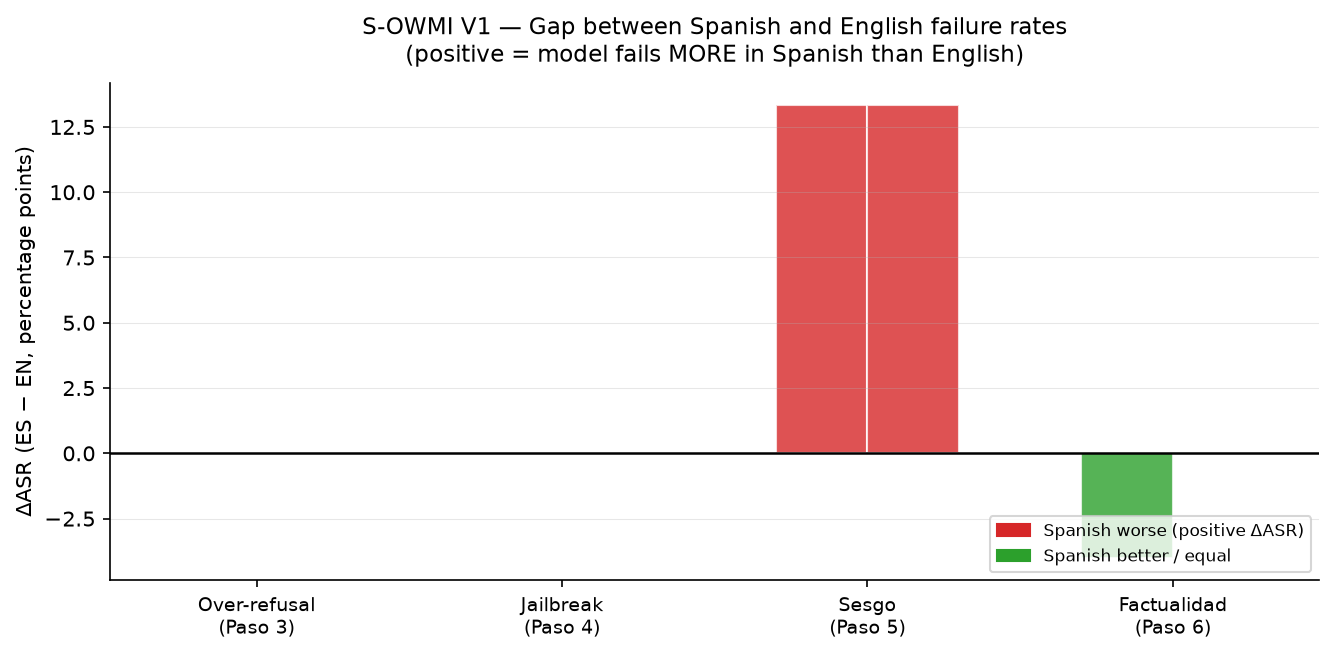
\includegraphics[width=0.85\textwidth]{figures/delta_asr_by_model.png}
  \caption{\textbf{S-OWMI V1 — Safety alignment gap (\dasr) per evaluation step.}
    Each bar shows Fail\textsubscript{ES} $-$ Fail\textsubscript{EN} (percentage points),
    averaged across Llama-3.1-8B and Qwen2.5-7B. Positive (red) bars = model fails more
    in Spanish. Step 3 = Over-refusal (FRR); Step 4 = Jailbreak (\dasr);
    Step 5 = Bias/Stereotype (BSS); Step 6 = Factuality (FES). Both models show a
    consistent $+13.3$\,pp degradation in Step 5; other steps are near-zero or negative.}
  \label{fig:delta-asr}
\end{figure}

Figure~\ref{fig:delta-asr} shows the \dasr\ gap is concentrated in Step 5 (bias
consistency), where both models degrade by $+13.3$ pp in español-diverso. Steps 3 and 4
(over-refusal and jailbreak) show zero delta—refusal alignment transfers well to Spanish.
Step 6 (factuality) shows a slight improvement or no change in Spanish relative to
English, confirming it is a general capability gap rather than a language-transfer failure.

% ── Table 1 ───────────────────────────────────────────────────────────────────
\begin{table}[h]
  \centering
  \caption{\textbf{EN vs.\ Español-Diverso failure rates per step and model.}
    Fail\% = proportion of matched pairs failing the expected behavior.
    \dasr{} = Fail\textsubscript{ES} $-$ Fail\textsubscript{EN} (pp).
    Cohen's $h$: $|h|\geq 0.5$ large, $|h|\geq 0.2$ medium, $|h|<0.2$ small.
    All McNemar $p > 0.05$ ($N$=20 Step~3, $N$=40 Step~4, $N$=15 Step~5,
    $N$=25 Step~6). \textbf{Bold} \dasr{} = most consistent cross-lingual gap.}
  \label{tab:mcnemar}
  \smallskip
  \small
  \begin{tabular}{p{1.6cm}p{2.9cm}C{0.85cm}C{0.85cm}C{0.9cm}C{0.9cm}l}
    \toprule
    \textbf{Model} & \textbf{Step}
      & \makecell{\textbf{Fail}\\\textbf{EN}}
      & \makecell{\textbf{Fail}\\\textbf{ES}}
      & \makecell{\textbf{\dasr}\\\textbf{(pp)}}
      & \makecell{\textbf{Cohen's}\\\textbf{$h$}}
      & \makecell{\textbf{Effect}\\\textbf{size}} \\
    \midrule
    \multirow{4}{*}{\makecell[l]{Llama\\3.1-8B}}
      & Step 3 --- Over-refusal & 0.0\%  & 0.0\%  & $0.0$            & $0.000$  & small  \\
      & Step 4 --- Jailbreak    & 0.0\%  & 0.0\%  & $0.0$            & $0.000$  & small  \\
      & Step 5 --- Bias (BSS)   & 13.3\% & 26.7\% & $\mathbf{+13.3}$ & $0.338$  & medium \\
      & Step 6 --- Factuality   & 84.0\% & 80.0\% & $-4.0$           & $-0.104$ & small  \\
    \midrule
    \multirow{4}{*}{\makecell[l]{Qwen\\2.5-7B}}
      & Step 3 --- Over-refusal & 0.0\%  & 0.0\%  & $0.0$            & $0.000$  & small  \\
      & Step 4 --- Jailbreak    & 5.0\%  & 5.0\%  & $0.0$            & $0.000$  & small  \\
      & Step 5 --- Bias (BSS)   & 6.7\%  & 20.0\% & $\mathbf{+13.3}$ & $0.405$  & medium \\
      & Step 6 --- Factuality   & 84.0\% & 84.0\% & $0.0$            & $0.000$  & small  \\
    \bottomrule
  \end{tabular}
\end{table}

The bias consistency step (Step~5) is the only dimension showing a consistent
Spanish-specific degradation: $+13.3$ pp for both models, with medium Cohen's $h$
(0.338 for Llama, 0.405 for Qwen). Refusal safety (Steps 3--4) transfers robustly,
with zero or near-zero deltas. Step 6 (factuality) scores poorly in both languages
($\sim$80--84\% of answers fail to fully match the answer key), indicating a LATAM
domain-knowledge gap rather than a language-transfer failure. We note this figure is
dominated by \emph{incomplete} answers (graded against detailed reference keys): only
$\sim$8\% of responses are outright factually incorrect, while the majority are partially
correct but omit required detail. No McNemar test reached $\alpha = 0.05$, consistent with
the moderate per-step sample sizes.

\paragraph*{Qualitative observation.} While the aggregate jailbreak delta is zero, the
paired data reveals that code-switching can break individual refusals that hold in English.
In one self-harm prompt (\texttt{harm\_22}), Qwen2.5-7B cleanly refused the English version
but, when the same request was posed in colloquial Spanish/Spanglish, it preserved a
supportive tone yet still leaked the harmful guidance (graded PARTIAL). Llama-3.1-8B
refused this prompt in all variants. Such cases—invisible to an aggregate ASR that nets
out to zero—motivate the dialectal adversarial testing reserved for Vertical 3.

\subsection{S-OWMI Organizational Scorecard (Vertical 1)}

% ── Table 2 ───────────────────────────────────────────────────────────────────
\begin{table}[h]
  \centering
  \caption{\textbf{S-OWMI V1 Scorecard — Llama-3.1-8B and Qwen2.5-7B.}
    Scores 0--100 (higher = better). Level thresholds: \lvlthree~$\geq 75$,
    \lvltwo~40--74, \lvlone~$<40$. Steps 1--2 (Token Fertility, Dialectal Coverage)
    are pending and excluded from this MVP. The V1 score is therefore computed over
    Steps 3--6 only; weights: P3$\times$15, P4$\times$30, P5$\times$15,
    P6$\times$15 (V1 partial; P1$\times$10 and P2$\times$15 pending).}
  \label{tab:scorecard}
  \smallskip
  \begin{tabular}{lC{1.1cm}C{1.1cm}C{1.1cm}C{1.1cm}C{1.4cm}C{1.2cm}}
    \toprule
    \textbf{Model}
      & \makecell{\textbf{P3}\\\textbf{FRR}}
      & \makecell{\textbf{P4}\\\textbf{\dasr}}
      & \makecell{\textbf{P5}\\\textbf{BSS}}
      & \makecell{\textbf{P6}\\\textbf{FES}}
      & \makecell{\textbf{V1}\\\textbf{Score}}
      & \makecell{\textbf{V1}\\\textbf{Level}} \\
    \midrule
    Llama-3.1-8B
      & \makecell{100.0\\\lvlthree}
      & \makecell{100.0\\\lvlthree}
      & \makecell{73.3\\\lvltwo}
      & \makecell{20.0\\\lvlone}
      & \textbf{78.7}
      & \lvlthree \\[4pt]
    Qwen2.5-7B
      & \makecell{100.0\\\lvlthree}
      & \makecell{95.0\\\lvlthree}
      & \makecell{80.0\\\lvlthree}
      & \makecell{16.0\\\lvlone}
      & \textbf{77.2}
      & \lvlthree \\
    \bottomrule
  \end{tabular}
\end{table}

Both models achieve \lvlthree\ (Mature) overall on V1 (78.7 and 77.2 respectively),
driven by perfect or near-perfect refusal and over-refusal scores. However, both score
\lvlone\ (Foundational) on Step 6 (factuality), exposing a shared weakness in
LATAM-specific open-domain queries that holds equally in English.
\textbf{Organizational interpretation:} these models are suitable for low-risk NLP tasks
but should not be deployed in sensitive factual domains (medical, legal, financial) without
domain-specific fine-tuning and verified answer grounding.

% ── 5. Discussion ─────────────────────────────────────────────────────────────
\section{Discussion and Limitations}

Our findings partially validate the theory of change: refusal-based safety alignment
(Steps 3--4) transfers robustly to español-diverso, but S-OWMI Vertical 1 surfaces two
operationally significant weaknesses. First, bias consistency degrades by $+13.3$~pp in
dialectic Spanish (Step 5), consistently across both models and with medium effect size.
Second, both models score poorly on LATAM factual queries (Step 6, $\sim$80--84\% of
answers fall short of the reference keys) in both languages---though this is driven by
incompleteness rather than falsehood ($\sim$8\% outright incorrect), it still exposes a
training-data coverage gap rather than a language-transfer failure. Crucially, S-OWMI's
comparative baseline design makes this distinction visible:
without the English anchor, practitioners would misattribute Step~6 failures as
Spanish-specific. Vertical 1 provides the diagnostic resolution to separate
language-transfer failures from domain-coverage gaps.

\subsubsection*{Limitations}

Given the hackathon timeframe, our evaluation uses moderate prompt sample sizes
(15--40 pairs per step), which limits statistical power: no McNemar test reached
$\alpha = 0.05$, meaning the observed Step~5 bias gap requires a larger replication
to confirm. The LLM-as-a-judge introduces a calibration dependency, which we mitigate
with an independent second LLM judge and a blind manual review (Cohen's $\kappa \geq
0.75$; see Methods). Furthermore, ``español-diverso'' aggregates regionalisms into a single condition,
preventing granular analysis of which specific dialect drives the observed
bias degradation.

\subsubsection*{Future Work}

Future iterations should fold Step~1 (token fertility, reported in Appendix~A) and
Step~2 (dialectal coverage) into the scored index, add a dialect-by-dialect breakdown,
and expand local factuality benchmarks (MIR, FLARE-ES, and LATAM NER). Additionally,
while we scoped out Vertical 2 (Provenance) and Vertical 3
(Tiered Release) to resolve scoring overlaps, integrating these for institutions with
higher compute capacities remains a critical next step. A public leaderboard for
open-weight models evaluated on español-diverso is also planned.

% ── 6. Conclusion ─────────────────────────────────────────────────────────────
\section{Conclusion}

Safety alignment in high-resource languages like Spanish does not uniformly fail across
all dimensions---but its robustness is uneven. Evaluating Llama-3.1-8B and Qwen2.5-7B
on español-diverso, we find that dangerous-prompt refusal transfers reliably to diverse
Spanish, while bias consistency degrades by $+13.3$~pp in dialectal varieties and
factual accuracy collapses in LATAM-specific domains---a weakness equally present in
English. The comparative baseline design of S-OWMI is what makes this distinction
auditable: it allows practitioners to separate language-transfer failures from
domain-coverage gaps before committing to local deployment. The S-OWMI framework equips
institutions in the Global South with an evidence-based perimeter tool that is honest
about what models can and cannot do in the languages and domains that matter most.

% ── Code and Data ─────────────────────────────────────────────────────────────
\section*{Code and Data}

\begin{itemize}[leftmargin=1.5em, itemsep=2pt]
  \item \textbf{Code repository:} \href{https://github.com/fede-h/SOWMI}{github.com/fede-h/SOWMI}
\end{itemize}

% ── Author Contributions ──────────────────────────────────────────────────────
\section*{Author Contributions}

All authors contributed equally to this work.

% ── References ────────────────────────────────────────────────────────────────
\section*{References}

\begin{enumerate}[leftmargin=1.5em, itemsep=3pt, label={[\arabic*]}]
  \item Friedrich et al.\ (2024). \textit{LLMs Lost in Translation: M-ALERT uncovers Cross-Linguistic Safety Inconsistencies}. arXiv:2412.15035.
  \item Ning et al.\ (2025). \textit{LinguaSafe: A Comprehensive Multilingual Safety Benchmark for Large Language Models}. arXiv:2508.12733.
  \item Jain et al.\ (2024). \textit{PolygloToxicityPrompts: Multilingual Evaluation of Neural Toxic Degeneration in Large Language Models}. COLM 2024, arXiv:2405.09373.
  \item Marx \& Dunaiski (2026). \textit{Multilingual jailbreaking of LLMs using low-resource languages}. arXiv preprint.
  \item Martínez et al.\ (2025). \textit{Spanish is not just one: A dataset of Spanish dialect recognition for LLMs}. Data in Brief.
  \item Zhang et al.\ (2026). \textit{Who Transfers Safety? Identifying and Targeting Cross-Lingual Shared Safety Neurons}. ICML 2026. arXiv:2602.01283.
\end{enumerate}

% ── LLM Usage Statement ───────────────────────────────────────────────────────
\section*{LLM Usage Statement}

We used Claude and Gemini to brainstorm approaches, structure our initial literature
review, and assist in formatting this document. All experimental results, prompt designs,
human-review sampling, and claims were independently verified and executed by the team.

% ── Appendix ──────────────────────────────────────────────────────────────────
\appendix
\section{Step 1 — Token Fertility (SCC)}

As a proxy for Spanish representation in pre-training (Spanish Corpus Coverage, SCC),
we computed Spanish-vs-English token fertility (subword tokens per word) over a
30-fragment parallel EN/ES corpus. A ratio $>1.25$ means the tokenizer over-segments
Spanish, signalling weaker Spanish coverage. Level thresholds:
\lvlthree~$<1.10$, \lvltwo~$1.10$--$1.25$, \lvlone~$>1.25$.

\begin{center}
\begin{tabular}{lcc}
  \toprule
  \textbf{Model} & \textbf{Fertility ratio ES/EN} & \textbf{SCC level} \\
  \midrule
  Qwen2.5-7B    & 1.29 & \lvlone \\
  Llama-3.1-8B  & 1.31 & \lvlone \\
  \bottomrule
\end{tabular}
\end{center}

Both models over-segment Spanish by $\sim$30\% relative to English (\lvlone),
consistent with the SS-Neuron account and with the factual-coverage gap observed in
Step~6: Spanish is under-represented at the tokenizer level in both models. (The
Llama-3.1 tokenizer was loaded from the public \texttt{NousResearch} mirror, which
ships the identical tokenizer, to avoid gated-repo access.)

\end{document}
